\section{Systematic uncertainties}
\label{sec:systematics}

The next subsections describe the for main sources of systematic uncertainties considered.
Other sources, which would matter in absolute quantities measurements,
cancel in the ratio between the rare and resonant channels. Table~\ref{tab:RKst_systematics}
summarises the various sources of systematics and their effect on the $R_{\Kstar}$ ratios.
The total systematic uncertainty is calculated as the square root sum of the single components.

\begin{table}[hb!]
\begin{center}
\caption{Summary of percent systematic uncertainties.}
\begin{tabular}{|c|c|c|}
\hline
Source              & 1--6 GeV$^2/c^4$ &  15--20 GeV$^2/c^4$ \\ \hline
Add swap            & 0.0         & 0.1    \\
Free misreco        & 0.3     &  --                                   \\
DCB                 & 0.7       & 1.3  \\

\hline

Eff.               & 2.1               & 2.4         \\
Bin migration      & 5.5                     & 6.9   \\

\hline

Total              & 5.9               & 7.3   \\

\hline 
\end{tabular}
\label{tab:RKst_systematics}
\end{center}
\end{table}



\subsection{Choice of PDF}

There is a certain arbitrariety in the choice of PDFs to model signal
and background contributions in the invariant mass fits, which could translate
in a bias on the final result. To asses this systematic the signal function
for the electron channels is varied from the default CB plus Gaussian to a Double Crystal
Ball function. This results in 
%negligible uncertainty on the $R_{\Kstar}$ measurement for
%the central-\qsq interval with respect to other sources and 
an uncertainty of $\sim0.1\%$ for the central-\qsq region and $\sim2.2\%$ for the high-\qsq interval.
Attempts to modify the PDF for the fit to muon channels result in a negligible systematic
with respect to what found for the electron channels.
The background PDF is changed in two ways. First of all a background component
is added using the shape of simulated events, where the kaon and pion IDs have been swapped.
Only the case in which this component is added both for the muon and electron channels is considered.
This adds a $\sim 1\%$ systematic uncertainty. Secondly, the misreconstructed background yield
in the rare electron channel if freed from its constrain to the background yield in the \jpsi sample.
This is only relevant for the electron channels as there is no misreconstructed
background in the muon ones. Furthermore, it is only relevant for the central-\qsq interval
as in the fit to high-\qsq candidates this yield is already free to float.
This results in a 1.4\% systematic uncertainty.

\subsection{Statistical error on the efficiency determination}

The statistical error on the determination of the efficiency is
considered as a source of systematic uncertainty. This is 
$\sim 1.5\%$ on $R_{ee}$ and $R_{\mu\mu}$ and, as it is due to fluctuations,
it does not cancel in their ratio. This yields $\sim2.5\%$ systematic uncertainty
on the $R_{\Kstar}$ measurement.
%, mainly coming from the determination of the trigger efficiency.


\subsection{TISTOS}

A further source of systematic, which is considered, is due to the
discrepancies found in Sec.~\ref{sec:tistos} on the determination of the trigger efficiency. 
As explained in that subsection the efficiency is derived as a function of the relevant
kinematic quantities for each trigger category. The efficiency
is then obtained for the rare and resonant sample by a weighted average.
These are found to be compatible indicating that the effect on the
ratios between rare and resonant channels is negligible.
Therefore, no systematic uncertainty is added for this source.
%The values found are compared between data and simulation and the full difference is
%added as a systematic uncertainty. This cancels out between electron and muon channels
%and yields an extra 0.2\% uncertainty at central \qsq and 1\% at high \qsq.


\subsection{Bin migration}

The determination of the reconstruction efficiency is affected by the knowledge of the
amount of bin migration as explained in Sec.~\ref{sec:reco_binmig}. This amount depends
on the shape of the \qsq distribution, which depends on the simulated model.
In order to asses this systematic, simulated samples are generated using different
models corresponding to different form factors~\cite{Ball:2004ye,Melikhov:2000yu}.
The generator level distributions obtained using each model are compared with the ones obtained using
the default one~\cite{Ali:1999mm}. These ratios are shown in Fig.~\ref{fig:q2ratios} as a function of \qsq
and are used to re-weight the simulation. The amount of bin migration is recalculated
using the simulation reweighted to reproduce each model.
Table~\ref{tab:sys_binmig} rep
orts the percent variation obtained with respect to the default model. 
The largest difference between two values is taken as systematic uncertainty.
This results in a $\sim5\%$ uncertainty for the central-\qsq interval and $\sim11\%$
for the high-\qsq one.
%
\begin{table}[h!]
\centering
\caption{Percent variation on the bin migration amount obtained using different form factors models.}
\begin{tabular}{|c|c|c|}
\hline
Model                   & 1--6 GeV$^2/c^4$  &  15--20 GeV$^2/c^4$ \\ \hline
Ball-Zwicky (6)         & 1.8          & 0.2    \\
Melikhov-Stech          & -3.7          & 6.6    \\
Colangelo QCD (3)   & 0.3           & 0.8    \\
Melikhov lattice  (4)   & -0.5          & -0.4    \\
\hline 
\end{tabular}
\label{tab:sys_binmig}
\end{table}

\begin{figure}[hb!]
\centering 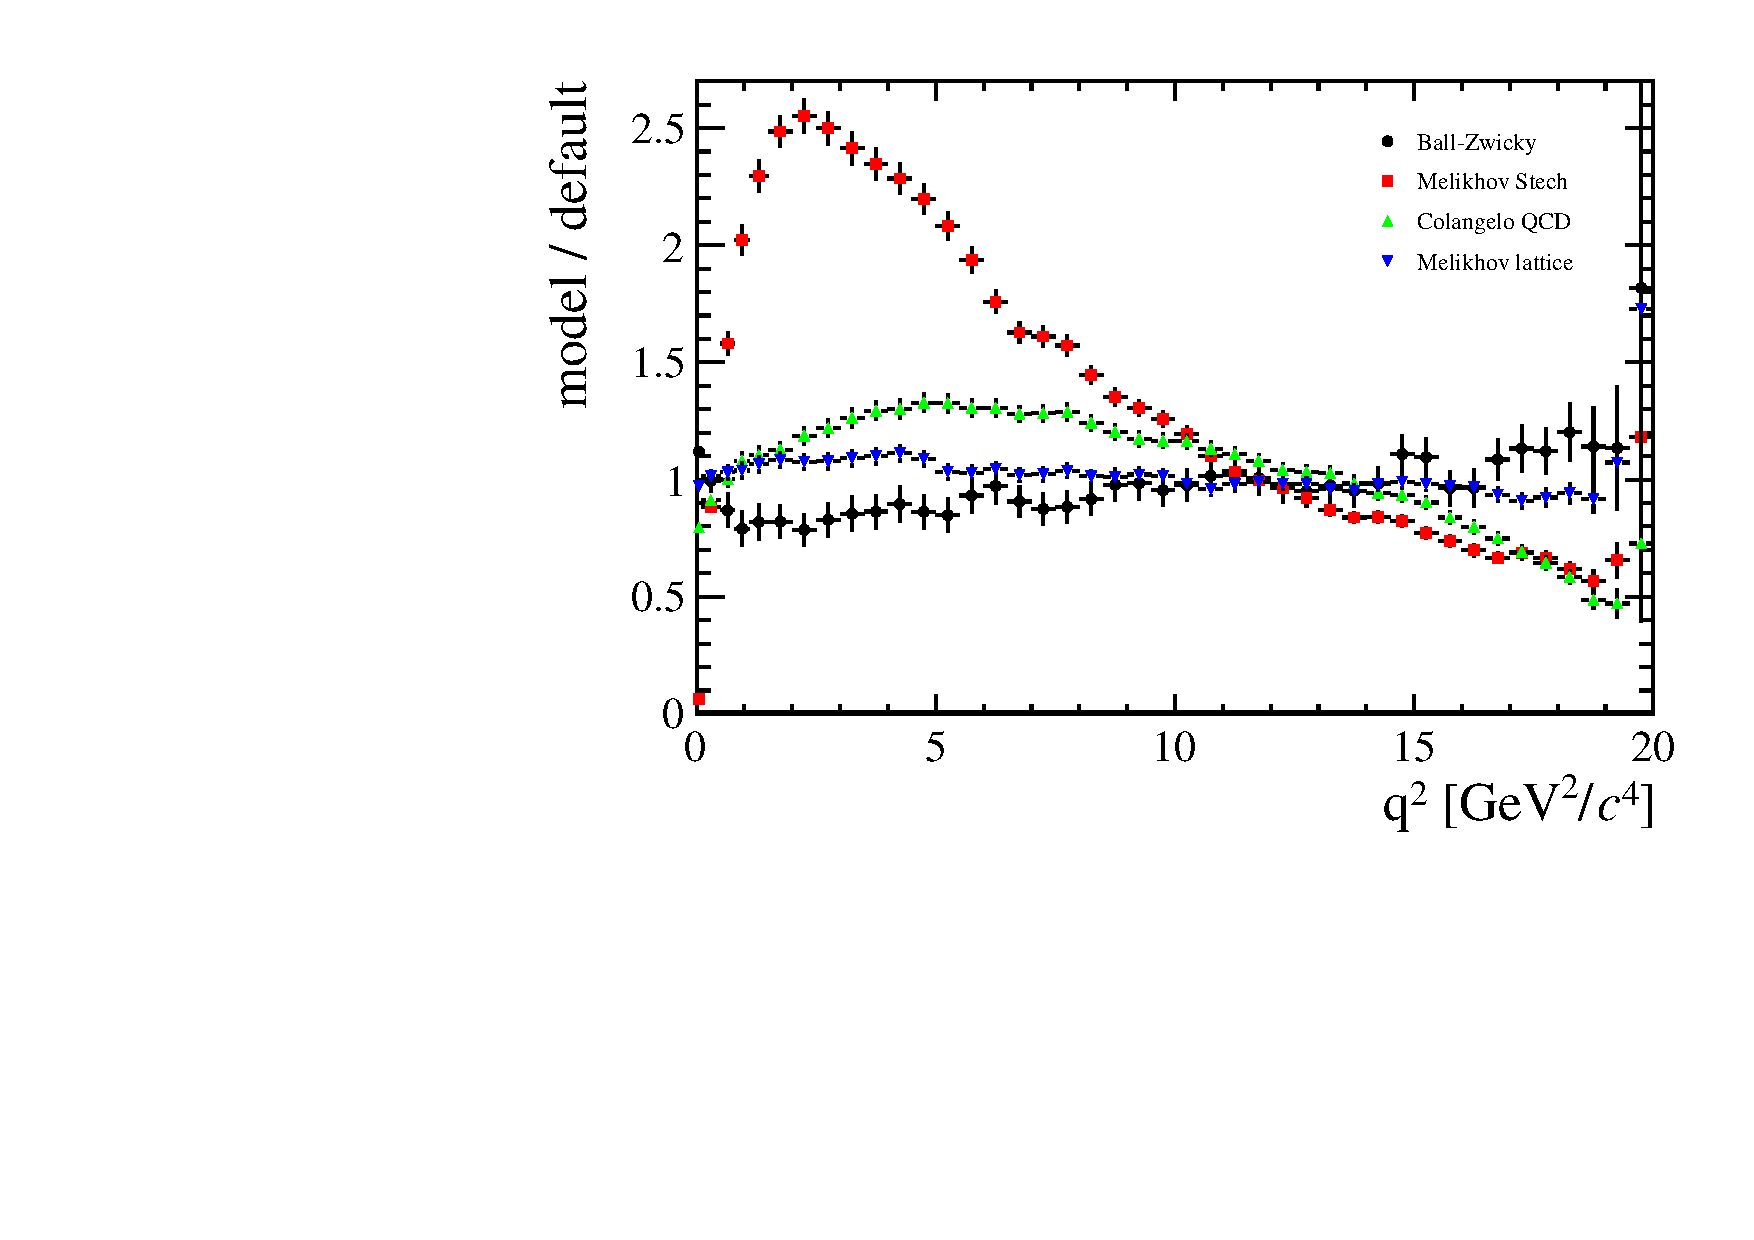
\includegraphics[width=0.8\textwidth]{RKst/figs/models_ratios.pdf}
\caption{Ratios between the \qsq distributions obtained using different form
factors models with respect to the default model. }
\label{fig:q2ratios}
\end{figure}



